% ===========================================================================
% Modèles de régression simples
% Traduit et adapté de :
%   https://www.bootstrapworld.org/materials/fall2026/en-us/lessons/regression-models-simple/
% Licence : Creative Commons 4.0 Unported (Bootstrap Community)
% ===========================================================================

\documentclass[12pt,a4paper]{article}

% ---------- Packages ----------
\usepackage[utf8]{inputenc}
\usepackage[T1]{fontenc}
\usepackage{libertine}
\usepackage{microtype}
\usepackage[french]{babel}
\usepackage{graphicx}
\usepackage{float}
\usepackage{hyperref}
\usepackage{geometry}
\usepackage{enumitem}
\usepackage{tabularx}
\usepackage{xcolor}
\usepackage{colortbl}
\usepackage[raster]{tcolorbox}
\usepackage{booktabs}
\usepackage{fancyhdr}
\usepackage{titlesec}
\usepackage{amsmath}
\usepackage{amssymb}
\usepackage{listings}

% ---------- Mise en page ----------
\geometry{margin=2.5cm, headheight=15pt, footskip=30pt}
\fancyhf{}
\fancyhead[L]{\textbf{Modèles de régression simples}}
\fancyhead[R]{\thepage}
\fancyfoot[C]{Bootstrap Community — CC BY 4.0}
\renewcommand{\headrulewidth}{0.4pt}
\pagestyle{fancy}

% ---------- Couleurs ----------
\definecolor{bsblue}{RGB}{41,128,185}
\definecolor{bsgreen}{RGB}{39,174,96}
\definecolor{bsorange}{RGB}{230,126,34}
\definecolor{bsgray}{RGB}{149,165,166}
\definecolor{codebg}{RGB}{245,247,250}

% ---------- Styles de sections ----------
\titleformat{\section}[hang]{\Huge\bfseries\color{bsblue}}{}{0pt}{}[\vspace{-0.5em}\rule{\textwidth}{2pt}]
\titleformat{\subsection}[hang]{\Large\bfseries\color{bsblue!80!black}}{}{0pt}{}
\titleformat{\subsubsection}[hang]{\large\bfseries\color{bsgreen!60!black}}{}{0pt}{}

% ---------- Environnements personnalisés ----------
\newtcolorbox{overviewbox}{
  colback=bsblue!5!white, colframe=bsblue!60!white,
  fonttitle=\bfseries, title=Objectif de la section,
  left=1em, right=1em, top=0.5em, bottom=0.5em
}
\newtcolorbox{activitybox}{
  colback=bsgreen!5!white, colframe=bsgreen!60!white,
  fonttitle=\bfseries, title=Activité,
  left=1em, right=1em, top=0.5em, bottom=0.5em
}
\newtcolorbox{thinkbox}{
  colback=bsorange!5!white, colframe=bsorange!60!white,
  fonttitle=\bfseries, title=Réflexion,
  left=1em, right=1em, top=0.5em, bottom=0.5em
}
\newtcolorbox{keypointbox}{
  colback=bsgray!10!white, colframe=bsgray!50!white,
  fonttitle=\bfseries, title=Point clé,
  left=1em, right=1em, top=0.5em, bottom=0.5em
}
\newtcolorbox{instructornotes}{
  colback=yellow!10!white, colframe=yellow!80!black,
  fonttitle=\bfseries, title=Notes pour l'enseignant·e,
  left=1em, right=1em, top=0.5em, bottom=0.5em
}
\newtcolorbox{codebox}{
  colback=codebg, colframe=bsgray!40,
  fonttitle=\bfseries, title=Code Pyret,
  left=1em, right=1em, top=0.5em, bottom=0.5em
}
\newtcolorbox{contractbox}{
  colback=bsblue!3!white, colframe=bsblue!40!white,
  left=1em, right=1em, top=0.6em, bottom=0.6em
}

% ---------- Style listings pour Pyret ----------
\lstdefinelanguage{Pyret}{
  keywords={use,context,url-file,and,or,not,if,else,for,fun,data,sharing,include,import,as,where,let,rec,is,=,true,false,end,Table,String,Number,Boolean,Image,Row,List,Code},
  sensitive=true,
  comment=[l]{\#},
  morestring=[b]",
  morestring=[b]',
}
\lstset{
  language=Pyret,
  basicstyle=\ttfamily\small,
  commentstyle=\color{bsgreen!70!black}\itshape,
  keywordstyle=\color{bsblue}\bfseries,
  stringstyle=\color{bsorange},
  backgroundcolor=\color{codebg},
  frame=single,
  framesep=5pt,
  rulecolor=\color{bsgray!40},
  breaklines=true,
  breakatwhitespace=false,
  showstringspaces=false,
  aboveskip=0.8em,
  belowskip=0.8em,
}

% ---------- Commandes pratiques ----------
\newcommand{\img}[3]{%
  \begin{figure}[H]
    \centering
    \includegraphics[#2]{#1}
    \caption{#3}
    \label{fig:#1}
  \end{figure}
}
\newcommand{\contrat}[1]{%
  \begin{contractbox}
    \ttfamily #1
  \end{contractbox}
}

% ---------- Informations du document ----------
\title{%
  \vspace{-2cm}
  {\Huge\bfseries Modèles de régression}\\[0.3em]
  {\Huge\bfseries simples}\\[0.5em]
  {\large Voitures autonomes, apprentissage supervisé et régression linéaire}\\[1em]
  {\normalsize Traduit et adapté depuis \href{https://www.bootstrapworld.org/materials/fall2026/en-us/lessons/regression-models-simple/}{Bootstrap World} (Fall 2026)}\\[0.5em]
  {\normalsize Licence Creative Commons 4.0 International}
}
\date{}
\author{}

\begin{document}

\maketitle
\thispagestyle{empty}

\vspace{2cm}
\begin{center}
  \textit{Ces supports ont été développés en partie grâce au soutien de la National Science Foundation\\
  (bourses 1042210, 1535276, 1648684, 1738598, 2031479 et 1501927).}
\end{center}

\newpage
\tableofcontents
\newpage

% ===========================================================================
% SECTION 1 : VOITURES AUTONOMES
% ===========================================================================
\section{Voitures autonomes}

\begin{overviewbox}
  Les élèves réfléchissent aux voitures autonomes comme exemple convaincant d'apprentissage automatique supervisé. Ils explorent un simulateur de conduite, collectent leurs propres données d'entraînement, et découvrent que prédire l'angle de braquage est un problème de régression.
\end{overviewbox}

% ---------- Launch ----------
\subsection{Lancement}

\img{images/c0b8e3daef30440c.jpg}{width=0.5\textwidth}{Une voiture autonome avec un capteur sur le toit, garée au milieu d'une route vide.}

Les voitures autonomes donnent l'impression que le futur est vraiment arrivé~! Beaucoup de gens pensent qu'elles sont l'un des meilleurs exemples d'«~IA~» qui pense vraiment, au lieu de «~suivre un algorithme~». Après tout, \emph{comment un ordinateur peut-il prendre des décisions sur la façon de conduire~?}

Laissez les élèves discuter. Rappelez-leur l'effet IA, et comment les gens ressentaient la même chose quand les premiers correcteurs orthographiques ont été développés~!

\begin{keypointbox}
  Les voitures autonomes fonctionnent grâce à de nombreuses entrées (capteurs, caméras, etc.) et de nombreuses sorties (combien accélérer, freiner, braquer). Le braquage, par exemple, est extrêmement difficile~! Les considérations incluent~:
  \begin{itemize}
    \item Si la route devant tourne à gauche ou à droite, et avec quelle netteté.
    \item La distance de la voiture par rapport au centre de la voie.
    \item Si la voiture est alignée avec la voie ou se dirige vers un côté.
    \item Les obstacles et feux de circulation qui pourraient se trouver sur le chemin.
    \item Et bien plus encore~!
  \end{itemize}

  Nous allons explorer comment une forme d'apprentissage supervisé — la \textbf{régression}, plus précisément — permet aux voitures de «~savoir où elles vont~».
\end{keypointbox}

\subsubsection{L'entraînement d'une voiture autonome}

Enseigner à une IA ce que signifie braquer nécessite un \textbf{entraînement}. Voici en quoi il consiste~:

\begin{enumerate}[leftmargin=*]
  \item \textbf{Une personne conduit le véhicule.}
  \begin{itemize}
    \item Dans l'apprentissage supervisé, le conducteur humain est souvent appelé le \emph{superviseur}.
    \item Le superviseur démontre le comportement correct (par exemple, dans quelle direction tourner le volant).
  \end{itemize}
  \item \textbf{Plusieurs fois par seconde, un ordinateur enregistre…}
  \begin{itemize}
    \item les informations de nombreux capteurs autour de la voiture~;
    \item la direction de braquage choisie par le conducteur à cet instant.
  \end{itemize}
  \item \textbf{Les données d'entraînement (le corpus d'entraînement) sont représentées comme une table entrée-sortie}, avec des colonnes pour les données des capteurs (entrées) et les angles de braquage corrects (sorties). Par exemple~:
\end{enumerate}

\begin{center}
\begin{tabular}{l l l}
  \toprule
  \texttt{curve} & \texttt{speed} & \texttt{steering-angle} \\
  \midrule
  1$^\circ$  & 45 & 0,02$^\circ$ \\
  4$^\circ$  & 21 & 55,20$^\circ$ \\
  $-$2$^\circ$ & 56 & $-$25,43$^\circ$ \\
  \bottomrule
\end{tabular}
\end{center}

\begin{enumerate}[leftmargin=*, resume]
  \item \textbf{Le jeu de données sert à générer une fonction.}
  \begin{itemize}
    \item La fonction prédit l'angle de braquage à partir des données des capteurs. Dans la table ci-dessus, \texttt{curve} et \texttt{speed} sont les variables explicatives~; \texttt{steering-angle} est la variable de réponse.
  \end{itemize}
  \item \textbf{Une fois l'entraînement terminé, un humain appuie sur le bouton «~run~» et le véhicule commence à conduire~!} Au fur et à mesure que la voiture roule, elle évalue continuellement sa fonction apprise pour produire des angles de braquage — tout comme le conducteur humain le faisait pendant l'entraînement.
\end{enumerate}

\begin{instructornotes}
  Si vous voulez montrer à vos élèves un exemple de voiture autonome précoce (1989~!), c'est le bon moment pour visionner \href{https://www.youtube.com/watch?v=ntIczNQKfjQ}{cette courte vidéo de deux minutes} du Robotics Institute de Carnegie Mellon University.
\end{instructornotes}

\begin{thinkbox}
  \begin{itemize}
    \item \textbf{Quelles autres entrées de capteur pourraient nous aider à déterminer l'angle de braquage souhaité~?}
    \begin{itemize}
      \item Dans quelle voie nous sommes, si la voiture est alignée avec la route, les obstacles sur notre chemin…
    \end{itemize}
    \item \textbf{L'apprentissage supervisé implique qu'un ordinateur apprend \emph{de} quelque chose. De quoi l'ordinateur apprend-il, dans notre exemple~?}
    \begin{itemize}
      \item D'un conducteur humain — le superviseur — qui a démontré le braquage correct.
      \item Ces paires entrée-sortie forment le corpus d'entraînement.
    \end{itemize}
    \item \textbf{Pourquoi le modèle résultant est-il une \emph{fonction}~?}
    \begin{itemize}
      \item Pour le même ensemble d'entrées (données des capteurs), le modèle doit toujours prédire la même sortie (angle de braquage).
    \end{itemize}
    \item \textbf{Pourquoi appelle-t-on cela de l'apprentissage \emph{supervisé}~?}
    \begin{itemize}
      \item Parce qu'un humain a fourni les bonnes réponses (angles de braquage) pendant l'entraînement, «~supervisant~» ce que la machine a appris.
    \end{itemize}
  \end{itemize}
\end{thinkbox}

\begin{keypointbox}
  \textbf{Les trois phases de l'apprentissage supervisé}
  \begin{enumerate}
    \item Des données étiquetées par des humains sont enregistrées, démontrant les connaissances à apprendre.
    \item Un algorithme d'apprentissage automatique trouve une \textbf{fonction} qui fait correspondre les entrées aux sorties correctes (la «~clé de réponses~»).
    \item La fonction apprise peut être appliquée à de nouvelles données, jamais vues auparavant.
  \end{enumerate}
\end{keypointbox}

% ---------- Investigate: Simulator ----------
\subsection{Exploration~: le simulateur de conduite}

\begin{activitybox}
  \begin{itemize}
    \item Ouvrez le fichier \textbf{Voiture Autonome — Fichier de Démarrage} (\texttt{Voiture\allowbreak-Autonome\allowbreak-Starter.arr}) et enregistrez une copie. Cliquez sur «~Run~».
    \item Tournez-vous vers \emph{Explorer le simulateur de conduite} et suivez les instructions.
  \end{itemize}

  Laissez les élèves jouer avec le simulateur pendant plusieurs minutes avant de débriefer. Les élèves qui terminent tôt peuvent essayer de collecter des données à différentes vitesses, ou conduire délibérément mal pour voir à quoi ressemble de mauvaises données d'entraînement.
\end{activitybox}

\begin{thinkbox}
  \begin{itemize}
    \item \textbf{Quelles colonnes avez-vous vues dans votre table de données d'entraînement~?}
    \begin{itemize}
      \item \texttt{speed}, \texttt{curve}, \texttt{skew}, \texttt{offset}, et \texttt{steering-angle}
    \end{itemize}
    \item \textbf{Quelle est la différence entre un \texttt{steering-angle} positif et négatif~?}
    \begin{itemize}
      \item Positif = tourner à droite. Négatif = tourner à gauche.
      \item (Cela pourrait être l'inverse pour d'autres simulateurs, selon la convention.)
    \end{itemize}
    \item \textbf{Combien de lignes de données avez-vous collectées en quelques minutes de conduite~?}
    \begin{itemize}
      \item probablement 500 à 1000.
    \end{itemize}
    \item \textbf{Entraîner un modèle de conduite nécessite les meilleures données possibles. Pensez-vous que vous ou quelqu'un d'autre pourriez mieux conduire la voiture sur la piste avec plus de pratique~?}
    \begin{itemize}
      \item Probablement~!
    \end{itemize}
  \end{itemize}
\end{thinkbox}

\begin{instructornotes}
  Nous avons préparé pour vous un corpus d'entraînement contenant des données de conduite expertes, collectées sur différentes conditions routières et vitesses de conduite. Il est déjà chargé dans le fichier de démarrage sous le nom \texttt{training}.

  \vspace{0.3em}
  \textbf{D'où vient \texttt{training}~?}

  Ce jeu de données a commencé comme des données réelles d'une course très lente et prudente sur plusieurs pistes. La taille initiale était un peu plus de 10~000~lignes, assemblées à partir de passages «~idéaux~» séparés sur plusieurs pistes. Les données brutes combinées ont ensuite été \emph{post-traitées} via une \href{https://fr.wikipedia.org/wiki/Moyenne_mobile}{moyenne mobile}, qui lisse les valeurs extrêmes en quelque chose de beaucoup plus naturel. Une autre étape de post-traitement a impliqué la suppression des valeurs aberrantes les plus sévères, en utilisant la connaissance de la piste (un \texttt{skew} supérieur à 80$^\circ$, par exemple, représente de toute évidence une erreur humaine~!).

  Nous avons même fourni une API pour que vos élèves puissent faire une partie de ce post-traitement eux-mêmes~:

  \contrat{\# trim :: (Table t, String col, Number lo, Number hi) -> Table\\
\# Étant donné une colonne, supprime toutes les lignes où la valeur dans cette colonne est en dehors de l'intervalle [lo, hi]}

  \contrat{\# sample-rows :: (Table t, Number every-n) -> Table\\
\# Étant donné une table, ne garde qu'une ligne sur n (utile pour ce jeu de données, où 5 lignes consécutives sont si proches dans le temps que les données supplémentaires ne sont que du bruit)}

  Est-ce de la «~triche~»~? Pas du tout~! En fait, c'est un excellent point de discussion si vos élèves le demandent. L'apprentissage automatique dépend tellement de la qualité des données que des efforts énormes sont consacrés à trouver des moyens d'améliorer cette qualité par toutes les méthodes disponibles, avant qu'un modèle ne soit entraîné.
\end{instructornotes}

% ---------- Synthesize ----------
\subsection{Synthèse}

\begin{thinkbox}
  \begin{itemize}
    \item \textbf{Pourquoi qualifie-t-on le processus d'entraînement d'une voiture autonque d'apprentissage supervisé~?}
    \begin{itemize}
      \item Parce que la colonne cible de notre jeu de données est un enregistrement de ce que les humains feraient en recevant les valeurs des autres colonnes.
    \end{itemize}
  \end{itemize}
\end{thinkbox}

\newpage

% ===========================================================================
% SECTION 2 : PRÉDIRE L'ANGLE DE BRAQUAGE
% ===========================================================================
\section{Prédire l'angle de braquage}

\begin{overviewbox}
  Les élèves identifient les variables explicatives candidates du corpus d'entraînement, créent des nuages de points pour explorer la relation entre chaque variable et \texttt{steering-angle}, et choisissent \texttt{curve} comme meilleur prédicteur unique.
\end{overviewbox}

% ---------- Launch ----------
\subsection{Lancement}

Dans la leçon \emph{Ajuster des modèles}, nous avons appris qu'une relation entre deux variables apparaît comme un nuage de points dans un diagramme de dispersion, et que nous pouvons décrire cette relation avec un modèle.

\begin{keypointbox}
  \begin{itemize}
    \item La \textbf{variable explicative} (axe des $x$) est l'entrée à partir de laquelle nous prédisons.
    \item La \textbf{variable de réponse} (axe des $y$) est ce que nous essayons de prédire.
  \end{itemize}

  Dans notre cas, la variable de réponse est \texttt{steering-angle}~: le nombre de degrés de rotation du volant. Les données d'entraînement ont plusieurs colonnes qui pourraient servir de variable explicative.
\end{keypointbox}

\subsubsection{Les quatre variables candidates}

\begin{center}
\begin{tabularx}{\textwidth}{l X}
  \toprule
  \textbf{Variable} & \textbf{Description} \\
  \midrule
  \texttt{curve}\par\noindent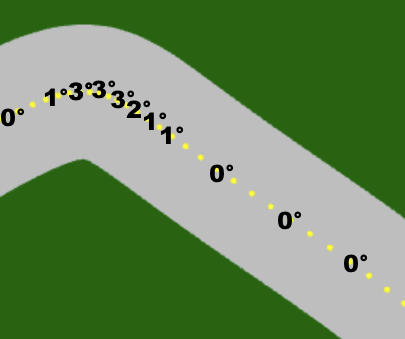
\includegraphics[width=0.35\textwidth]{images/6792236dd07b4b35.png} & La courbure de la route devant la voiture \\
  \texttt{speed}\par\noindent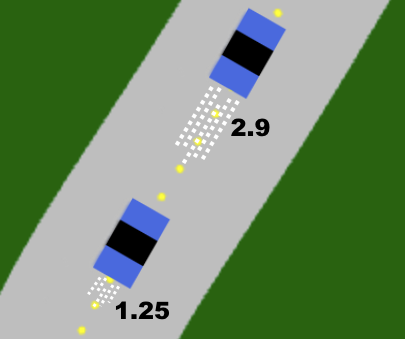
\includegraphics[width=0.35\textwidth]{images/92b6320812d86abe.png} & La vitesse à laquelle la voiture se déplace \\
  \texttt{offset}\par\noindent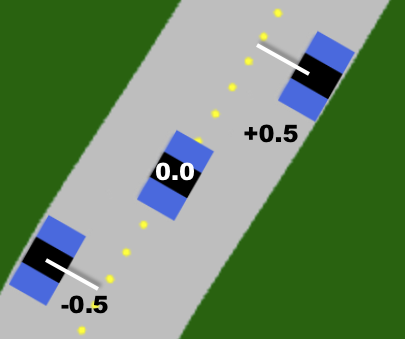
\includegraphics[width=0.35\textwidth]{images/53a610e925bbc0a1.png} & La distance de la voiture par rapport à la ligne centrale \\
  \texttt{skew}\par\noindent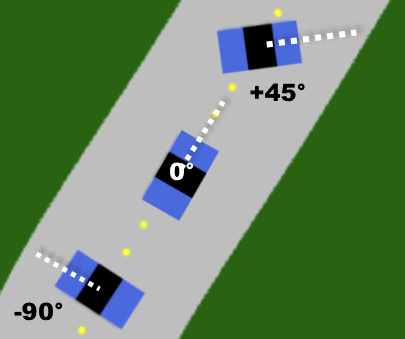
\includegraphics[width=0.35\textwidth]{images/53ac1798c81b74fd.png} & L'angle de la voiture par rapport à la route \\
  \bottomrule
\end{tabularx}
\end{center}

\begin{thinkbox}
  \begin{itemize}
    \item \textbf{Laquelle de ces variables pensez-vous être le meilleur prédicteur de l'angle de braquage, et pourquoi~?}
    \begin{itemize}
      \item Les réponses varieront — c'est destiné à stimuler la discussion et faire émerger les intuitions avant que les données ne parlent.
    \end{itemize}
  \end{itemize}
\end{thinkbox}

\begin{thinkbox}
  \begin{itemize}
    \item \textbf{Quelle visualisation de données fonctionne le mieux pour montrer les relations possibles entre deux variables quantitatives~?}
    \begin{itemize}
      \item Les nuages de points (\emph{scatter plots}).
    \end{itemize}
    \item \textbf{Que devons-nous chercher dans nos visualisations pour choisir la meilleure variable explicative~?}
    \begin{itemize}
      \item La relation la plus forte (points le plus étroitement regroupés autour d'une droite).
    \end{itemize}
  \end{itemize}
\end{thinkbox}

% ---------- Investigate: Scatter plots ----------
\subsection{Exploration~: nuages de points}

\begin{activitybox}
  \begin{itemize}
    \item Retournez au fichier \textbf{Voiture Autonome}.
    \item Utilisez \texttt{scatter-plot} pour comparer chacune des quatre colonnes explicatives possibles à \texttt{steering-angle}.
    \item Puis complétez \emph{Qu'est-ce qui prédit l'angle de braquage~?}.
  \end{itemize}
\end{activitybox}

\begin{instructornotes}
  Circulez et encouragez les élèves à lire les nuages de points de façon critique. Poussez-les à remarquer si la relation paraît linéaire, l'importance de la dispersion, et s'il y a des valeurs aberrantes évidentes.
\end{instructornotes}

\img{images/ffea137f9e29c5a9.png}{width=0.55\textwidth}{Nuage de points de \texttt{steering-angle} en fonction de \texttt{curve}, montrant une relation linéaire positive.}

\begin{thinkbox}
  \begin{itemize}
    \item \textbf{Quelle variable a montré la relation la \textbf{plus forte} avec \texttt{steering-angle}~?}
    \begin{itemize}
      \item \texttt{curve} a une relation claire, presque linéaire. Plus la route tourne fortement dans une direction, plus l'angle de braquage augmente proportionnellement.
    \end{itemize}
    \item \textbf{Quelle variable a montré la relation la \textbf{plus faible}~?}
    \begin{itemize}
      \item \texttt{speed} — il y a beaucoup de dispersion sans motif linéaire clair.
    \end{itemize}
    \item \textbf{Une des relations vous a-t-elle surpris~?}
    \begin{itemize}
      \item Les réponses varieront.
    \end{itemize}
  \end{itemize}
\end{thinkbox}

\begin{instructornotes}
  Si les élèves remarquent que le nuage de points pour \texttt{offset} a une image presque miroir du nuage de \texttt{curve} et pensent que c'est un prédicteur aussi bon~: attirez leur attention sur le fait que les plages des axes~$x$ pour \texttt{curve} et \texttt{offset} sont assez différentes. Réinitialisez la fenêtre du nuage de points \texttt{curve} à $-30 < x < 30$ (pour correspondre à la fenêtre de \texttt{offset}) afin qu'ils puissent voir que les données sont beaucoup plus étroitement regroupées pour \texttt{curve}.

  Si vous voulez donner à vos élèves plus de pratique avec \texttt{fit-model} et l'interprétation des valeurs~$S$, vous pouvez leur demander de définir les 4~modèles dans le fichier de démarrage et d'évaluer leur ajustement.
\end{instructornotes}

% ---------- Synthesize ----------
\subsection{Synthèse}

\begin{thinkbox}
  \begin{itemize}
    \item \textbf{Si vous n'aviez que 2~lignes de données d'entraînement — et qu'elles tombent en ligne droite parfaite — feriez-vous confiance à un modèle construit à partir de ces 2~points~?}
    \begin{itemize}
      \item Non — deux points peuvent \textbf{toujours} être reliés par une droite. Cela ne veut pas dire que le motif est réel ou se généralisera.
    \end{itemize}
    \item \textbf{Combien de données pensez-vous qu'il faudrait avant de pouvoir faire confiance à un modèle~?}
    \begin{itemize}
      \item Il n'y a pas de réponse unique, mais davantage de données collectées dans une plus grande variété de conditions rendent un modèle plus fiable.
    \end{itemize}
    \item \textbf{La taille du jeu de données est-elle le seul facteur important pour un bon jeu d'entraînement~?}
    \begin{itemize}
      \item Non — nous avons aussi besoin de données \emph{représentatives}~! Une voiture autonome doit être construite sur des données de toutes sortes de routes, conditions météo, offsets, heures de la journée, tailles de route, vitesses, densité de trafic, etc.
    \end{itemize}
  \end{itemize}
\end{thinkbox}

\newpage

% ===========================================================================
% SECTION 3 : RÉGRESSION LINÉAIRE
% ===========================================================================
\section{Régression linéaire}

\begin{overviewbox}
  Après avoir ajusté manuellement un modèle linéaire aux données, les élèves utilisent la fonction \texttt{lr-plot} de Pyret pour trouver l'ajustement optimal. Ils interprètent les coefficients du modèle et testent leurs prédicteurs avec la fonction \texttt{drive}. Enfin, ils réfléchissent à ce que signifie avoir «~entraîné~» un modèle.
\end{overviewbox}

% ---------- Launch ----------
\subsection{Lancement}

Dans \emph{Qu'est-ce qui prédit l'angle de braquage~?}, vous avez estimé la pente ($m$) et l'ordonnée à l'origine ($b$) des droites que vous avez ajustées aux nuages de points. Mais comment savoir si c'étaient les \emph{meilleurs} modèles linéaires — la droite de meilleur ajustement pour les données~?

\begin{keypointbox}
  Les data scientist·es utilisent une méthode appelée \textbf{régression linéaire} pour trouver le motif de droite qui décrit un ensemble d'entrées et une sortie cible déjà connue avec les valeurs \emph{mathématiquement optimales} de $m$ et $b$.

  \begin{itemize}
    \item Cette forme d'apprentissage — où nous connaissons déjà la sortie correcte pour chaque entrée — est appelée \textbf{apprentissage supervisé}.
    \item En apprentissage automatique, l'acte de trouver une fonction à partir des données est appelé \textbf{entraînement}.
  \end{itemize}

  Les modèles de régression linéaire minimisent l'erreur autant que possible.

  La fonction \texttt{lr-plot} de Pyret calcule et visualise la droite de meilleur ajustement. Son contrat est le même que \texttt{scatter-plot}~:

  \contrat{\# lr-plot :: (Table t, String labels, String xs, String ys) -> Image}
\end{keypointbox}

\begin{activitybox}
  \begin{itemize}
    \item Utilisez \texttt{lr-plot} sur \texttt{training} pour trouver la droite de meilleur ajustement pour chacune des variables comparées à \texttt{steering-angle}.
    \item Comment les modèles optimaux de Pyret pour les données se comparent-ils à ceux que vous avez ajustés à la main~?
  \end{itemize}
\end{activitybox}

\begin{instructornotes}
  Les élèves remarqueront que \texttt{lr-plot} définit des modèles avec des valeurs décimales, certainement avec une spécificité supérieure à leur modèle dessiné à la main. Cela motive l'idée que l'ordinateur peut optimiser cela bien mieux et plus vite que les humains — ce qui est, après tout, le but de l'apprentissage automatique.
\end{instructornotes}

\img{images/63c0a48efc22a390.png}{width=0.55\textwidth}{Nuage de points de \texttt{steering-angle} en fonction de \texttt{curve}, montrant une relation linéaire positive. La droite de meilleur ajustement est superposée au nuage de points.}

\begin{thinkbox}
  \begin{itemize}
    \item \textbf{Que nous dit la pente de notre modèle \texttt{curve} ($\approx 19{,}5$)~?}
    \begin{itemize}
      \item Que l'angle de braquage augmente d'environ 19,5 degrés pour chaque augmentation de 1~degré de la courbure.
    \end{itemize}
    \item \textbf{Que nous dit l'ordonnée à l'origine de notre modèle \texttt{curve} ($\approx 0{,}41$)~?}
    \begin{itemize}
      \item Si la courbure est nulle, l'angle de braquage devrait être de 0,41$^\circ$.
    \end{itemize}
    \item \textbf{Est-ce que cela a du sens dans le monde réel~?}
    \begin{itemize}
      \item Presque. Une route avec zéro courbure devrait nécessiter zéro degré de braquage, mais au lieu de cela nous voyons un peu moins d'un demi-degré~!
    \end{itemize}
    \item \textbf{Que nous dit la valeur~$S$~?}
    \begin{itemize}
      \item Nous nous attendons à ce que l'erreur des prédictions de ce modèle soit de l'ordre de 37~degrés.
      \item Cela pourrait expliquer ce mystérieux braquage de 0,41$^\circ$ quand la route est droite~!
    \end{itemize}
  \end{itemize}
\end{thinkbox}

\begin{thinkbox}
  \begin{itemize}
    \item \textbf{Sur la base de la valeur~$S$, vous attendez-vous à ce que le modèle \texttt{curve} puisse réussir à «~conduire~» un tour complet de piste~?}
    \begin{itemize}
      \item Probablement pas~! 37~degrés est une erreur assez importante.
    \end{itemize}
    \item \textbf{Nos fonctions de prédiction s'attendent-elles à ce que l'angle de braquage augmente quand nos autres variables augmentent~?}
    \begin{itemize}
      \item Non~! L'angle de braquage devrait diminuer quand \texttt{skew} et \texttt{offset} augmentent.
    \end{itemize}
    \item \textbf{Comment un modèle de régression est-il «~avec perte~» (\emph{lossy})~? Quels détails des données d'entraînement originales perd-il~?}
    \begin{itemize}
      \item Tout ce qui est au-dessus ou en dessous de la droite de régression est une donnée réelle, que nous écartons quand nous utilisons la droite.
    \end{itemize}
  \end{itemize}
\end{thinkbox}

\begin{instructornotes}
  Nous ne pouvons pas calculer un $S$ \emph{significatif} si nous n'avons pas plus de deux lignes dans notre table~!

  Une droite passant par deux points les ajuste tous les deux parfaitement, donc notre valeur $S$ est zéro. Mais cela en dit moins sur le modèle que sur le manque de données~: il n'y a pas d'erreur à mesurer, donc c'est un «~ajustement parfait~» sans vraie signification.
\end{instructornotes}

% ---------- Investigate: drive function ----------
\subsection{Exploration~: la fonction \texttt{drive}}

Voyons comment nos prédicteurs conduisent la voiture~! Pyret possède une fonction \texttt{drive}~:

\contrat{\# drive :: (predictor :: Row -> Number) -> Table\\
\# fait tourner le simulateur de conduite, en utilisant \emph{predictor} pour calculer l'angle de braquage à chaque image}

\begin{activitybox}
  \begin{enumerate}
    \item Remarquez que \texttt{drive} prend une fonction qui consomme une \textbf{Row} — mais \texttt{pred-c} consomme un \textbf{Number}, pas une Row~!
    \item \textbf{Pourquoi \texttt{drive} a-t-il besoin d'une fonction consommant une Row plutôt qu'un Number~?}
    \begin{itemize}
      \item Parce qu'à chaque instant, \texttt{drive} a accès à toute la ligne de données — pas juste une colonne. Une fonction consommant une Row peut décider quelles colonnes regarder.
    \end{itemize}
    \item \textbf{Comment pouvons-nous obtenir une version de \texttt{pred-c} qui consomme une Row~?}
    \begin{itemize}
      \item Nous pourrions l'écrire à la main, mais Pyret a exactement l'outil qu'il faut~:
    \end{itemize}
  \end{enumerate}
\end{activitybox}

\contrat{\# regression-model-code :: (Table t, List<String> inputs, String prediction) -> Code\\
\# produit le code qui définit un modèle entraîné consommant une Row\\
\# (à copier/coller dans la Zone de Définitions~!)}

\begin{codebox}
Par exemple~:
\begin{lstlisting}
regression-model-code(training, [list: "curve"], "steering-angle")
  \end{lstlisting}
\end{codebox}

\img{images/bb2026a7194ff4df.png}{width=0.45\textwidth}{ALVINN / Navlab, une ambulance militaire reconvertie en voiture autonome.}

\begin{activitybox}
  \begin{itemize}
    \item Copiez et collez la définition \texttt{curve-predictor} que vous venez de générer dans votre Zone de Définitions et cliquez sur «~Run~» pour la charger. Puis évaluez \texttt{drive(curve-predictor)} dans la Zone d'Interactions.
    \item Utilisez \texttt{regression-model-code} pour générer un prédicteur consommant une Row pour chacune des autres variables.
    \item Copiez et collez les définitions résultantes de \texttt{offset-predictor}, \texttt{skew-predictor}, et \texttt{speed-predictor} dans votre Zone de Définitions. Cliquez sur «~Run~».
    \item Essayez chacune avec \texttt{drive(...)}.
  \end{itemize}

  \begin{itemize}
    \item \textbf{Quel prédicteur conduisait le mieux~? Cela correspondait-il à vos prédictions des nuages de points~?}
    \begin{itemize}
      \item \texttt{curve-predictor} — oui, il avait la relation linéaire la plus forte avec \texttt{steering-angle}.
    \end{itemize}
    \item \textbf{Le prédicteur conduisait-il mieux que vous~? Pourquoi~?}
    \begin{itemize}
      \item Non~!
      \item Quand nous conduisions, nous pouvions prendre en compte toutes les variables, alors que le prédicteur n'en utilisait qu'une seule.
    \end{itemize}
  \end{itemize}
\end{activitybox}

\begin{instructornotes}
  \textbf{Idées fausses courantes}

  \textbf{Les données d'entraînement peuvent ne pas être représentatives du monde réel~!} Les élèves peuvent s'attendre à ce qu'un prédicteur construit à partir de bonnes données de braquage conduise parfaitement. Rappelez-leur qu'un modèle ne peut généraliser qu'à partir de ce qu'il a vu — il n'a aucune compréhension de la route. Des données d'une conduite parfaite sur une route droite produiront un modèle qui pourrait très mal s'en sortir sur une route sinueuse~!

  \vspace{0.3em}
  \textbf{Programmation avancée}

  Si vous enseignez dans le contexte d'un cours d'informatique, vous pouvez demander aux élèves de trouver comment rendre leur fonction \texttt{pred-c} capable de consommer une \texttt{Row} au lieu d'un \texttt{Number}. C'est un excellent exercice sur l'abstraction et la notion de structure de données, utilisant des outils de programmation qu'ils ont vus dans les leçons précédentes.

  Si vos objectifs d'apprentissage portent davantage sur la culture IA ou les mathématiques, ce serait un bon défi pour un élève avancé. Sinon, vous pouvez passer à \texttt{regression-model-code}, qui écrira le code d'accès aux Row à leur place.
\end{instructornotes}

% ---------- Synthesize ----------
\subsection{Synthèse}

\begin{keypointbox}
  Félicitations — vous venez d'\textbf{entraîner un modèle d'apprentissage automatique~!}

  \begin{itemize}
    \item \textbf{Que signifiait «~entraîner~» dans ce contexte~?}
    \begin{itemize}
      \item Nous avons fourni à l'ordinateur un jeu de données de paires entrée-sortie (\texttt{curve} $\to$ \texttt{steering-angle}), et il a trouvé la fonction qui fait le mieux correspondre entrée et sortie.
    \end{itemize}
    \item \textbf{Supposons que la voiture rencontre une courbe plus forte que toutes celles des données d'entraînement. Que fera le prédicteur~?}
    \begin{itemize}
      \item Il extrapolera à partir du motif qu'il a appris — ce qui peut ou non être précis. Il n'a aucun moyen de savoir qu'il est en dehors de sa plage d'entraînement.
    \end{itemize}
    \item \textbf{Et si nos données d'entraînement ont toutes été collectées sur des routes sèches, et que la voiture conduit maintenant sur de la glace~?}
    \begin{itemize}
      \item Le modèle n'a jamais été entraîné sur ces conditions. Il prédira comme si les conditions étaient normales — ce qui pourrait être très faux.
    \end{itemize}
  \end{itemize}
\end{keypointbox}

\begin{thinkbox}
  \begin{itemize}
    \item \textbf{Pourrions-nous entraîner un modèle en utilisant plus d'une variable explicative~?}
    \begin{itemize}
      \item Oui~! La régression multiple permet de prédire une variable de réponse à partir de plusieurs variables explicatives.
    \end{itemize}
    \item \textbf{À quoi ressemblerait une droite de meilleur ajustement sur un nuage de points avec \emph{deux} variables explicatives~? Aurions-nous une pente et une ordonnée~? Deux~?}
    \begin{itemize}
      \item La droite deviendrait un \emph{plan} dans un espace 3D, avec une pente pour chaque variable explicative.
    \end{itemize}
  \end{itemize}
\end{thinkbox}

\begin{keypointbox}
  \textbf{Les ordinateurs ne sont pas des gens~!}

  Dans les conversations sur l'IA, les ordinateurs sont souvent \emph{anthropomorphisés} — on leur prête des traits humains alors qu'ils ne sont pas humains. Cela peut empêcher les élèves de comprendre la mécanique de l'apprentissage automatique.

  Évitez de dire que le modèle «~sait~» conduire, ou qu'il «~comprend~» la route.

  Le résultat d'un modèle est toujours le fruit d'une \textbf{computation mathématique} — l'évaluation d'une fonction apprise sur une entrée. Tout l'apprentissage automatique supervisé repose sur des données, des fonctions, et des computations.
\end{keypointbox}

\newpage

% ===========================================================================
% ANNEXES
% ===========================================================================
\section*{Annexe A~: Le vocabulaire de l'apprentissage supervisé}

\begin{center}
\begin{tabularx}{\textwidth}{l X}
  \toprule
  \textbf{Terme} & \textbf{Définition} \\
  \midrule
  Apprentissage supervisé & Forme d'apprentissage où l'algorithme apprend à partir d'exemples étiquetés (entrées avec sorties connues), fournis par un superviseur humain. \\
  Corpus d'entraînement & L'ensemble des données étiquetées utilisées pour entraîner le modèle. \\
  Entraînement & L'acte de trouver une fonction à partir des données d'entraînement. \\
  Modèle & Une fonction qui résume la relation entre les variables d'entrée et de sortie. \\
  Variable explicative & L'entrée utilisée pour prédire la sortie (axe des $x$). Aussi appelée variable indépendante. \\
  Variable de réponse & La sortie que nous essayons de prédire (axe des $y$). Aussi appelée variable dépendante. \\
  Régression linéaire & Méthode statistique qui trouve la droite de meilleur ajustement entre une variable explicative et une variable de réponse. \\
  Droite de meilleur ajustement & La droite qui minimise la somme des résidus au carré. \\
  Résidu & La différence entre la valeur réelle et la valeur prédite par le modèle, pour un point donné. \\
  $S$ (écart-type des résidus) & Mesure de la qualité d'ajustement~: plus $S$ est petit, meilleur est l'ajustement. Exprimé en unités de la variable de réponse. \\
  Surapprentissage & Quand un modèle «~mémorise~» le bruit des données d'entraînement au lieu d'apprendre le motif réel, et échoue sur de nouvelles données. \\
  \bottomrule
\end{tabularx}
\end{center}

\section*{Annexe B~: Fichiers du projet}

\begin{center}
\begin{tabularx}{\textwidth}{l X}
  \toprule
  \textbf{Fichier} & \textbf{Description} \\
  \midrule
  \texttt{Voiture\allowbreak-Autonome\allowbreak-Starter.arr} & Fichier de démarrage Pyret~: charge \texttt{self\allowbreak-driving\allowbreak-car\allowbreak-library.arr} depuis Bootstrap, fournit \texttt{training}, \texttt{drive}, \texttt{lr-plot}, \texttt{regression\allowbreak-model\allowbreak-code}, etc. \\
  \texttt{modeles-regression-simples.tex} & Document de cours (ce fichier) \\
  \texttt{images/} & Photos (voiture autonome, ALVINN/Navlab) et diagrammes (courbure, vitesse, offset, skew, nuages de points) \\
  \bottomrule
\end{tabularx}
\end{center}

\vspace{1em}
\textbf{À noter~:} contrairement aux leçons précédentes (arbres de décision, ajustement de modèles), ce fichier de démarrage ne charge pas de données CSV externe. La table \texttt{training} est fournie \emph{directement} par la bibliothèque \texttt{self-driving-car-library.arr} de Bootstrap. Les noms de colonnes (\texttt{steering-angle}, \texttt{curve}, \texttt{speed}, \texttt{skew}, \texttt{offset}) sont codés en dur dans la bibliothèque et ne peuvent pas être traduits sans modifier la bibliothèque elle-même (744 lignes). Tous les commentaires et noms de fonctions définis par l'élève sont en français.

\section*{À propos de ces supports}

Ces supports ont été développés en partie grâce au soutien de la \emph{National Science Foundation} (bourses 1042210, 1535276, 1648684, 1738598, 2031479 et 1501927).

\begin{center}
  \textbf{Bootstrap} par la Communauté Bootstrap est sous licence Creative Commons 4.0 Unported.\\
  Cette licence n'accorde pas la permission d'organiser des formations ou du développement professionnel.\\[1em]
  \textit{Traduction et adaptation française réalisées en juillet 2026.}\\
  \textit{Source originale~: \url{https://www.bootstrapworld.org/materials/fall2026/en-us/lessons/regression-models-simple/}}
\end{center}

\end{document}